\documentclass[10pt,pdf,hyperref={unicode},xcolor=dvipsnames]{beamer}

\usepackage{float}
\usepackage{amsmath}
\usepackage{amsfonts}
\usepackage{bbm}

% русский текст в формулах?
\usepackage{mathtext}

\usepackage{booktabs} % toprule/bottomrule

% русский
\usepackage[T2A]{fontenc}
\usepackage[russian]{babel}
\usepackage[utf8]{inputenc}

% рисунки
\usepackage{graphicx, caption, subcaption}

\usetheme{CambridgeUS}

\usepackage{csquotes}
\usepackage[backend=bibtex]{biblatex}
\bibliography{biblio}

\usepackage{physics}
\usepackage{braket}

\usepackage{siunitx}
\sisetup{output-exponent-marker=\ensuremath{\mathrm{e}}}

% ?
\setbeamertemplate{frametitle}[default][center]

\addtobeamertemplate{navigation symbols}{}{%
\usebeamerfont{footline}%
\usebeamercolor[fg]{footline}%
\hspace{1em}%
\large\insertframenumber/\inserttotalframenumber
}

\newcommand{\mytitle}[1]{\color{blue}{\textbf{#1}}}

\newcommand{\lb}{\left(}
\newcommand{\rb}{\right)}
\newcommand{\lsq}{\left[}
\newcommand{\rsq}{\right]}

\usepackage{dsfont}
\usepackage{bbm}

\newcommand{\bbA}{\mathbb{A}}
\newcommand{\bbB}{\mathbb{B}}
\newcommand{\bbV}{\mathbb{V}}
\newcommand{\bbH}{\mathbb{H}}

\newcommand{\lc}{\left\{}
\newcommand{\rc}{\right\}}

\newcommand{\psip}[1]{\psi^{(#1)}(x)}
\newcommand{\fx}[0]{f(x)}
\newcommand{\psix}[0]{\psi(x)}

\newcommand{\hD}{\hat{D}}

% slightly modifying gather environment
\let\oldgather\gather
\def\gather{\vspace*{-0.2cm}\oldgather}

\begin{document}

\begin{frame}{\center\mytitle{\Large Конечно-разностные матричные методы. \\ Расчет колебательно-вращательных уровней в двухатомной молекуле. \\ Сравнение классической и квантовой статистических сумм.}}
\begin{table}[]
\flushright
\begin{tabular}{r}
\large Финенко Артем \\[1ex]
\end{tabular}
\end{table}
\vfill
\center
\today
\end{frame}

\begin{frame}{Структура доклада}
    \begin{block}{}
        \begin{itemize}
            \item Основные подходы к нахождению колебательно-вращательных уровней в двухатомной молекуле \\ 
            \item Метод Нумерова и его матричный аналог \\
            \item Метод Нумерова и трехточечная формула. Аналитические результаты \\ 
            \item Обобщенный матричный метод Нумерова \\
            \item Экстраполяция Ричардсона для собственных значений \\
            \item Альтернативный способ получения матричных задач. \\
            \item Расчет колебательно-вращательных уровней в потенциале Морзе. Сравнение с BOUND. \\
            \item Расчет статистических сумм \\
        \end{itemize}
    \end{block}
\end{frame}

\begin{frame}{Основные подходы к одномерному уравнению Шредингера}
    \centering
   
    \begin{figure}[H]
        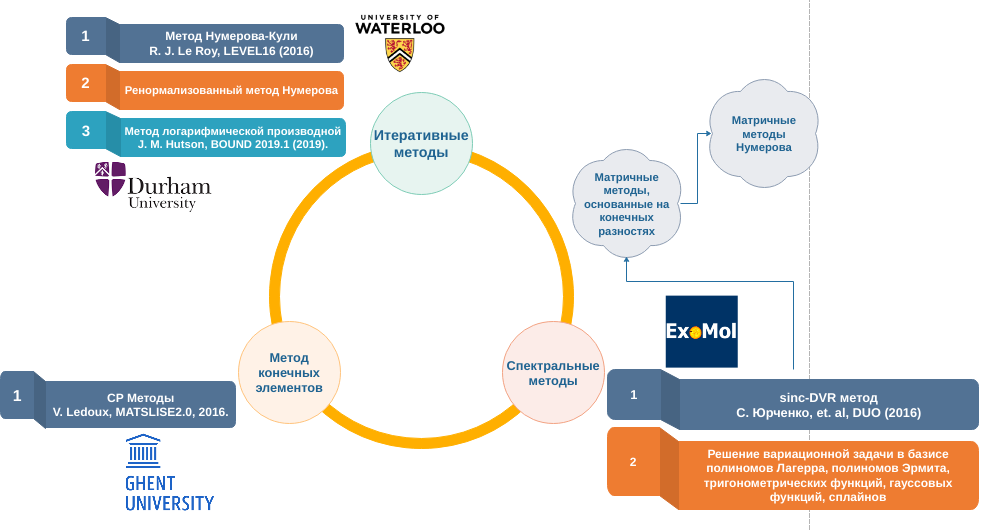
\includegraphics[width=\linewidth]{./pictures/diagram.png}
    \end{figure}
\end{frame}

\begin{frame}{Метод Нумерова и его матричный аналог}
    \begin{block}{}
        Метод Нумерова -- численный метод, позволяющий решать дифференциальные уравнения второго порядка\footnote{Метод Нумерова допускает ненулевой свободный член в ДУ}
        \begin{gather}
            \psip{2} = f(x) \psi(x), \quad f(x) = -\frac{2 m}{\hbar^2}\lsq E - V(x) \rsq, \quad \psip{n} = \frac{d^n}{dx^n} \psi(x).
        \end{gather}
        Используя Тейлоровское разложение для волновой функции
        \begin{gather}
            \hspace*{-0.1cm}
            \psi(x \pm h) = \psi(x) \pm h \psip{1} + \frac{1}{2!} h^2 \psip{2} \pm \frac{1}{3!} h^3 \psip{3} + \frac{1}{4!} h^4 \psip{4} + O(h^5), \notag
        \end{gather}
        получим выражение для второй производной $\psip{2}$ с точностью до $O(h^4)$
        \begin{gather}
            \psip{2} = \frac{ \psi(x+h) + \psi(x-h) - 2\psi(x) }{ h^2 } - \frac{1}{12} h^2 \psip{4} + O ( h^4 ).
        \end{gather}
    \end{block}
\end{frame}

\begin{frame}{Метод Нумерова и его матричный аналог}
    \begin{block}{}
        Используем это выражение для получения четвертой производной $\psip{4}$ с точностью до $O(h^2)$
        \begin{gather}
            \psip{4} = \frac{d^2}{dx^2} \psip{2} = \frac{d^2}{dx^2} \lsq \fx \psix \rsq = \notag \\
                     = \frac{ f(x+h)\psi(x+h) + f(x-h)\psi(x-h) - 2f(x)\psi(x) }{ h^2 } + O(h^2). 
        \end{gather}
        Подставляем в выражение для второй производной (суммарный порядок остается $O(h^4)$)
        \begin{gather}
            \fx \psix = \frac{\psi(x+h)+\psi(x-h)-2\psi(x)}{h^2} - \hspace{5cm} \notag \\ 
            - \frac{f(x+h) \psi(x+h) + f(x-h) \psi(x-h) - 2f(x) \psi(x)}{12} + O(h^4).
        \end{gather}
    \end{block}
\end{frame}

\begin{frame}{Метод Нумерова и его матричный аналог}
    \begin{block}{}
        При пропагировании на сетке используют вспомогательную функцию 
        \begin{gather}
            \omega(x) =  \lb 1 - \frac{h^2}{12} \rb \psi(x) \\
            \omega(x + h) = 2\omega(x) - \omega(x-h) + h^2 f(x) \psi(x).
        \end{gather}
        Вводя обозначения
        \begin{gather}
            V_{i-1} \equiv V(x-h), \quad V_i \equiv V(x), \quad V_{i+1} \equiv V(x + h) \\
            \psi_{i - 1} \equiv \psi(x-h), \quad \psi_i \equiv \psi(x), \quad \psi_{i+1} \equiv \psi(x+h),
        \end{gather}
        получаем следующее выражение, удобное для матричной техники 
        \begin{gather}
            \hspace*{-0.3cm}
            -\frac{\hbar^2}{2 m} \frac{\psi_{i+1} + \psi_{i-1} - 2 \psi_i}{h^2} + \frac{V_{i+1} \psi_{i+1} + V_{i-1}\psi_{i-1}+10 V_i \psi_i}{12} = E \frac{\psi_{i-1} + 10 \psi_i + \psi_{i+1}}{12}. \notag 
        \end{gather}
    \end{block}
\end{frame}

\begin{frame}{Метод Нумерова и его матричный аналог}
    \begin{block}{}
        Матричная формулировка метода Нумерова 
        \begin{gather}
            -\frac{\hbar^2}{2 m} \bbA \psi + \bbB \bbV \psi = E \bbB \psi, \quad \psi(a) = 0, \psi(b) = 0 \\
            a = x_0 < x_1 < \dots < x_{n-1} < x_n = b, \quad h = \frac{b - a}{n} \\
            \psi = \lsq \psi_i, i = 1 \dots n - 1 \rsq^\top, \quad \bbV = \text{diag} \left\{ V_i, i = 1 \dots n - 1 \right\} \\
            \bbA = \frac{1}{h^2} 
            \begin{bmatrix}
                -2 & 1 & 0 & 0 & \dots \\
                 1 &-2 & 1 & 0 & \dots \\ 
                 0 & 1 & -2& 1 & \dots \\
                 0 & 0 & 1 & -2& \dots \\
                 \vdots & \vdots & \vdots & \vdots & \ddots
            \end{bmatrix}, \quad
            \bbB = \frac{1}{12} 
            \begin{bmatrix}
                10 & 1 & 0 & 0 & \dots \\
                1 & 10 & 1 & 0 & \dots \\
                0 & 1 & 10 & 1 & \dots \\
                0 & 0 & 1 & 10 & \dots \\
                \vdots & \vdots & \vdots & \vdots & \ddots
            \end{bmatrix} \\
            \bbH \psi = E \psi, \quad \bbH = -\frac{\hbar^2}{2m} \bbB^{-1} \bbA + \bbV
        \end{gather}
    \end{block}
\end{frame}

\begin{frame}{Трехточечная оценка второй производной}
    \begin{block}{}
        Использование трехточечной формулы для оценки второй производной $\psip{2}$ приводит к матричной задаче, похожей на Нумеровскую \footfullcite{goorvitch1992}
        \begin{gather}
            -\frac{ \hbar^2 }{ 2m } \psip{2} + V(x) \psi(x) = E \psi(x), \\
            \psip{2} = \frac{\psi(x+h) + \psi(x-h) - 2\psi(x)}{h^2} + O(h^2) \\
            \bbH = - \frac{\hbar^2}{2m} \bbA + \bbV \\
            \bbA = \frac{1}{h^2} 
            \begin{bmatrix}
                -2 & 1 & 0 & 0 & \dots \\
                1 & -2 & 1 & 0 & \dots \\
                0 & 1 & -2 & 1 & \dots \\
                \vdots & \vdots & \vdots & \vdots & \ddots
            \end{bmatrix}
        \end{gather}
    \end{block}
\end{frame}

\begin{frame}{Трехточечная оценка и метод Нумерова}
    \begin{block}{}
        Набор собственных значений $\lc \lambda_k \rc_{k=1}^n$ мы приближаем набором собственных значений $\lc \lambda_k^{(N)} \rc_{k=1}^{n}$ матрицы $\bbH$ размерности $N$. \par 
        Если потенциальная энергия $V \in C^{(2)}[a, b]$, то разница между приближенным $k$-ым собственным значением  по матричной трехточечной формуле и его точным значением ведет себя как $\vert \lambda_k - \lambda_k^{(N)} \vert = O( k^4 h^2 )$ \footfullcite{paine1981}. При $V \equiv 0$:
        \begin{gather}
            \vert \lambda_k - \lambda_k^{(N)} \vert = k^2 - \frac{4}{h^2} \sin^2 \lb \frac{k h}{2} \rb = -\frac{1}{12} h^2 k^4 + \frac{1}{360} h^4 k^6 + O(h^6 k^8)
        \end{gather}
        Если потенциальная энергия $V \in C^{(4)}[a, b]$, то та же разница для матричного метода Нумерова ведет себя как $\vert \lambda_k - \lambda_k^{(N)} \vert = O(h^4)$ \footfullcite{andrew1986}.
    \end{block}
\end{frame}

\begin{frame}{Трехточечная оценка и метод Нумерова}
    \vspace*{-0.35cm}
    \begin{block}{Гармонический осциллятор, нулевой уровень, аппроксимация порядка по шагу $h$, $N = 40-400$}
        \begin{figure}[H]
            \centering
            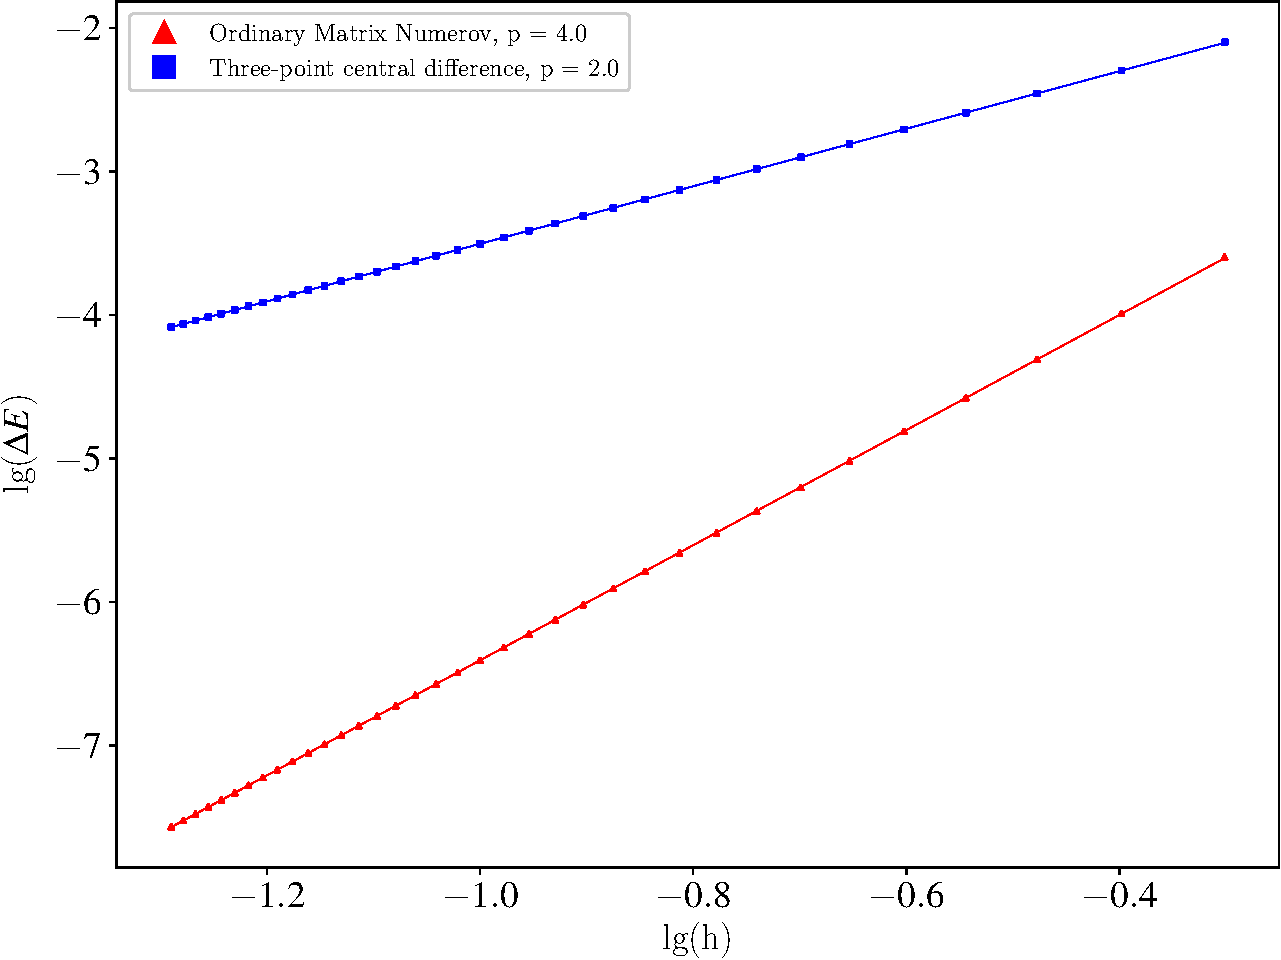
\includegraphics[width=0.75\linewidth]{./pictures/4numerov_vs_3point-crop.pdf}
        \end{figure}
    \end{block}
\end{frame}

\begin{frame}{Обобщенный метод Нумерова \footfullcite{dongjiao2014}}
    \begin{block}{}
        \vspace*{-0.5cm}
        Для получения метода порядка $N = 2r + 2$, выразим вторую производную $\psip{2}$ с точностью до порядка $N + 2$ 
        \begin{gather}
            \psi(x+h) + \psi(x-h) = 2 \psi(x) + \sum_{k=1}^{r+1} \frac{ 2h^{2k} }{ (2k)! } \psip{2k} + O(h^{2r+4}), \\
            \psip{2} = \frac{ \psi(x+h) + \psi(x-h) - 2\psi(x) }{ h^2 }  - \sum_{k=0}^{r-1} \frac{ 2h^{2k+2} }{ (2k+4)! } \psip{2k+4} + O(h^{2r+2}). \notag
        \end{gather}
        Неизвестными являются производные $\lc \psip{2k + 4}, k = 0 \dots r-1 \rc$, которые мы найдем из системы линейных уравнений
        \begin{gather}
            \lc
            \begin{aligned}
                \frac{ \psi(x+h) + \psi(x-h) - 2\psi(x) }{ 2 } &= \sum_{k=1}^{r} \frac{ h^{2k} }{ (2k)! } \psip{2k} + O(h^{2r+2}) \\ 
                                                               &\dots \\
                \frac{ \psi(x+r\cdot h) + \psi(x-r \cdot h) - 2\psi(x) }{ 2 } &= \sum_{k=1}^{r} \frac{ (r \cdot h)^{2k} }{ (2k)! } \psip{2k} + O(h^{2r+2}) \\ 
            \end{aligned}
            \right.
        \end{gather}
    \end{block}
\end{frame}

\begin{frame}{Обобщенный метод Нумерова}
    \begin{block}{}
        \vspace*{-0.5cm}
        В результате решения линейной системы получаем наборы коэффициентов $\lc c_i \rc_{i=1}^r$, $\lc k_i \rc_{i=1}^r$, позволяющие получить выражения
        \begin{gather}
            \psip{2} = \frac{1}{h^2} \sum_{i=-r}^r c_i \psi_i - \frac{2 h^{2r}}{(2r+2)!} \psip{2r+2} + O(h^{2r+2}) \\
            \psip{2r} = \frac{1}{h^{2r}} \sum_{i=-r}^r k_i \psi_i 
        \end{gather}
        Воспользуемся приемом из стандратного метода Нумерова для нахождения $\psip{2r+2}$
        \begin{gather}
            \psip{2r+2} = \frac{d^r}{dx^r} \lb f(x) \psi(x) \rb = \frac{1}{ h^{2r} } \sum_{i=-r}^r k_i f_i \psi_i.
        \end{gather}
        Собирая полученные выражения, получаем уравнения обобщенного метода Нумерова 
            \vspace*{-0.4cm}
        \begin{gather}
            \frac{1}{h^2} \sum_{i=-r}^r c_i \psi_i = f_i \psi_i + \sum_{i=-r}^r \frac{2}{(2r+2)!} k_i f_i \psi_i.
        \end{gather}
    \end{block}
\end{frame}

\begin{frame}{Обобщенный метод Нумерова}
    \begin{block}{Пример. Порядок $N = 8, (r = 3)$.}
        \vspace*{-0.5cm}
        \begin{gather}
            \bbH \psi = E \psi, \quad \bbH = -\frac{\hbar^2}{2m} \bbB^{-1} \bbA + \bbV \\
            \bbA = \frac{1}{180h^2}
            \begin{bmatrix}
                490 & 270 & -27 & 2 & 0 & \dots \\
                270 & 490 & 270 & -27 & 2 & \dots \\
                -27 & 270 & 490 & 270 & -27 & \dots \\
                  2 & -27 & 270 & 490 & 270 & \dots \\
                  0 & 2   & -27 & 270 & 490 & \dots \\
                  \vdots & \vdots & \vdots & \vdots & \vdots & \ddots
            \end{bmatrix}, \\
            \bbB = \frac{1}{20160}
            \begin{bmatrix}
                20140 & 15 & -6 & 1 & 0 & \dots \\
                15 & 20140 & 15 & -6 & 1 & \dots \\
                -6 & 15 & 20140 & 15 & -6 & \dots \\
                1 & -6 & 15 & 20140 & 15 & \dots \\
                0 & 1 & -6 & 15 & 20140 & \dots \\
                \vdots & \vdots & \vdots & \vdots & \vdots & \ddots
            \end{bmatrix}
        \end{gather}
    \end{block}
\end{frame}

\begin{frame}{Асимптотика по размеру шага}
    \vspace*{-0.5cm}
    \begin{block}{Гармонический осциллятор, нулевое состояние, $N=40-400$}
        \begin{figure}[H]
            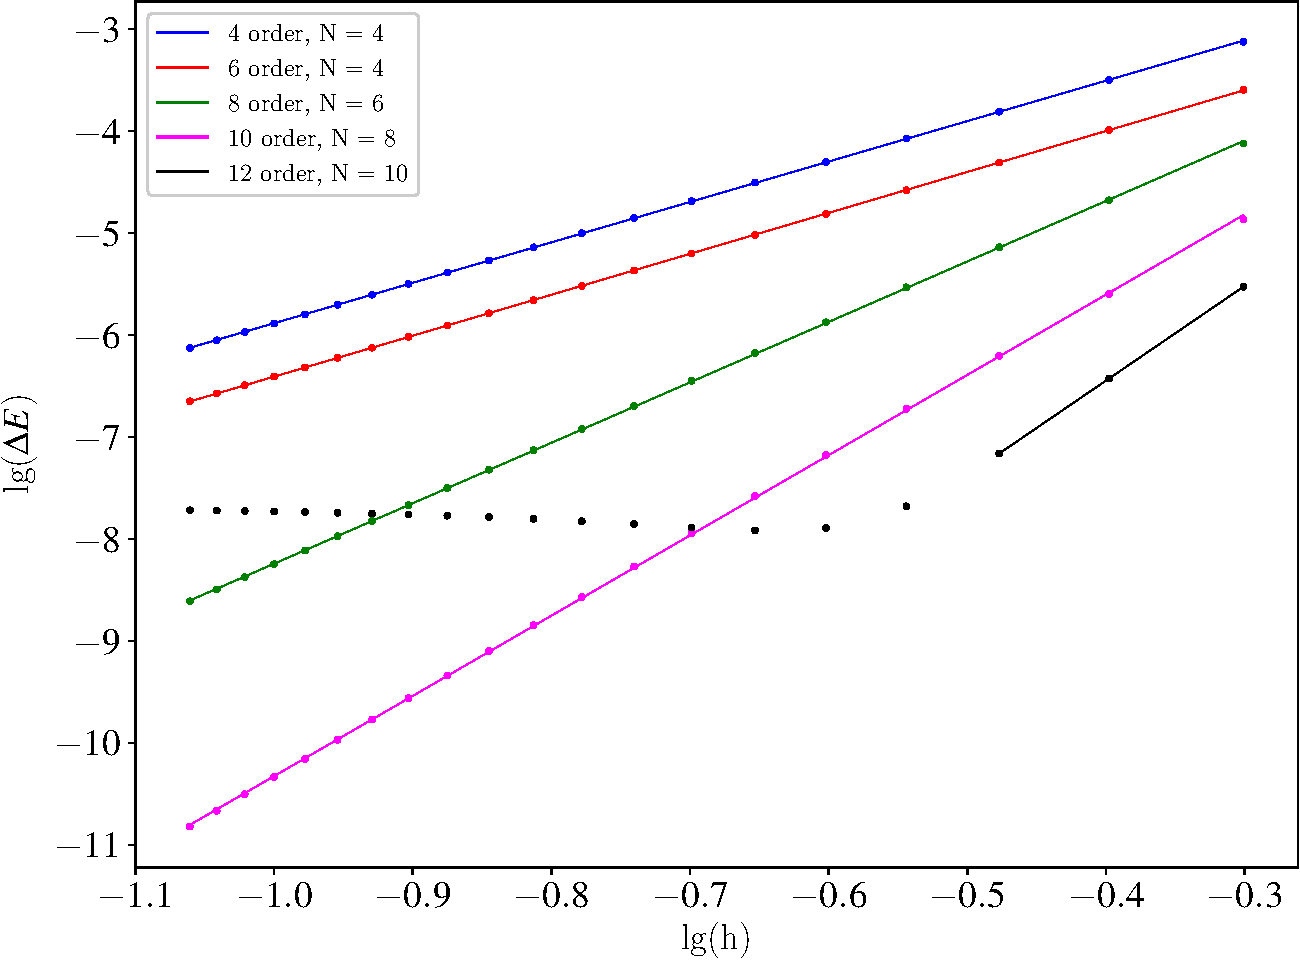
\includegraphics[width=0.8\linewidth]{./pictures/diff_h-crop.pdf}
        \end{figure}
    \end{block}
\end{frame}

\begin{frame}{Асимптотика по номеру состояния}
    \vspace*{-0.5cm}
    \begin{block}{Гармонический осциллятор, $n = 400$}
        \begin{figure}[H]
            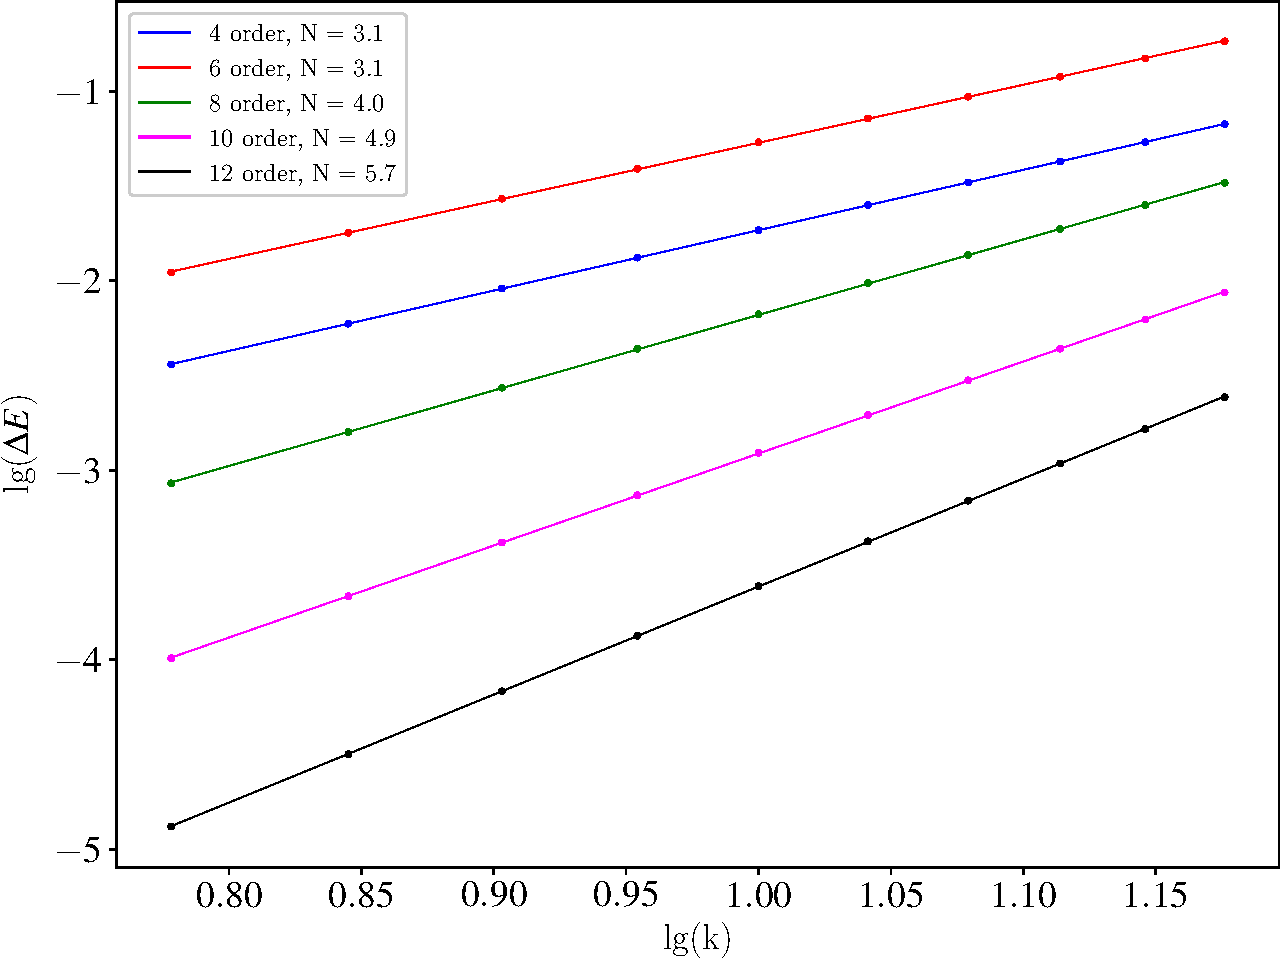
\includegraphics[width=0.8\linewidth]{./pictures/diff_k-crop.pdf}
        \end{figure}
    \end{block}
\end{frame}

\begin{frame}{Асимптотика по номеру состояния}
    \vspace*{-0.5cm}
    \begin{block}{Гармонический осциллятор, $n = 400$}
        \begin{figure}[H]
            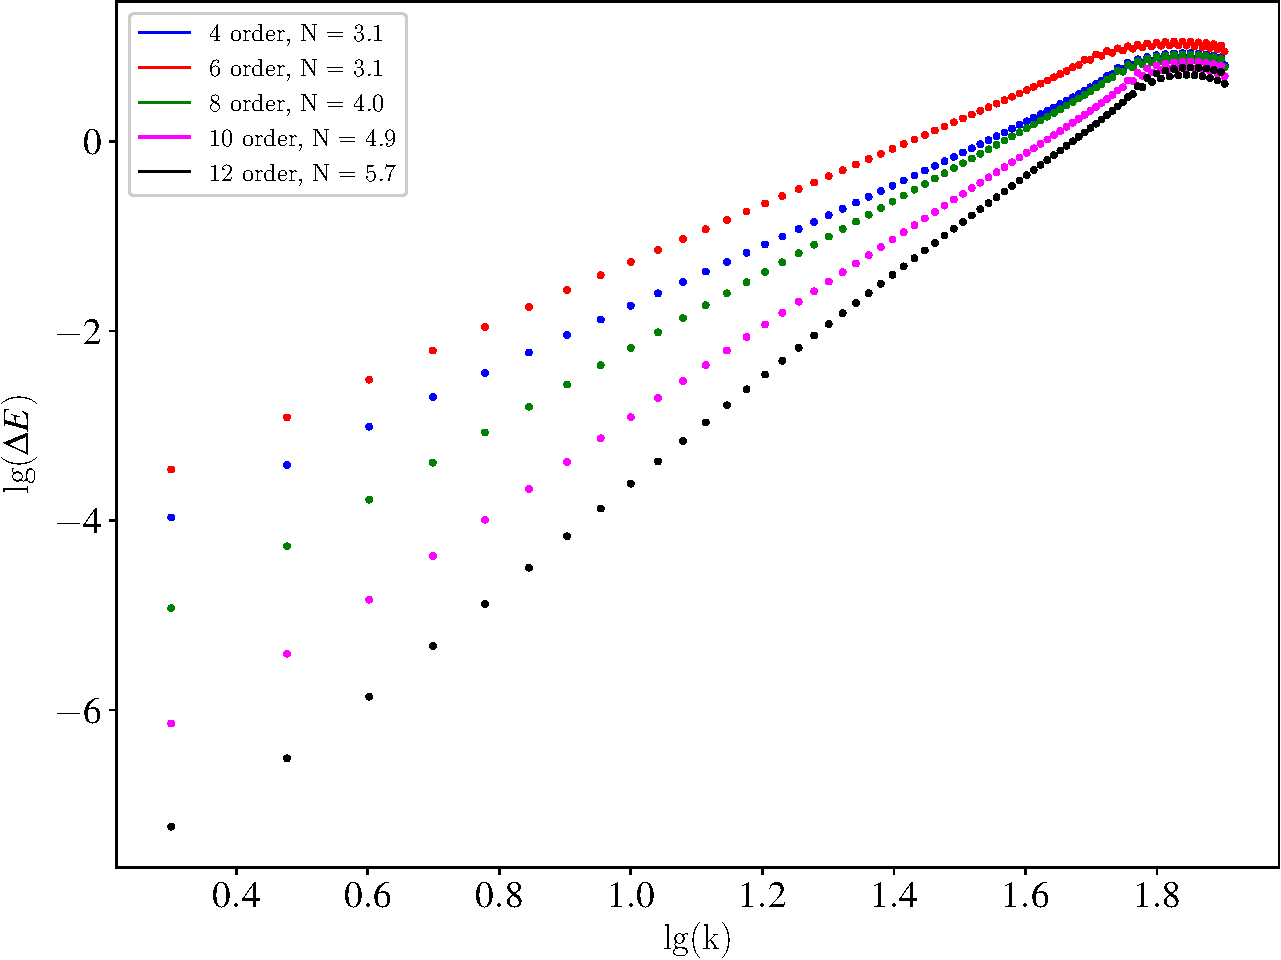
\includegraphics[width=0.8\linewidth]{./pictures/diff_k_nonlinear-crop.pdf}
        \end{figure}
    \end{block}
\end{frame}

\begin{frame}{Экстраполяция по Ричардсону}
    \vspace*{-0.5cm}
    \begin{block}{\enquote{Базельская задача}}
        \vspace*{-0.5cm}
        \begin{gather}
            \frac{\pi^2}{6} = \sum_{k=1}^\infty \frac{1}{k^2}, \quad S_N = \sum_{k=1}^N \frac{1}{k^2}
        \end{gather}
        Предположим следующее асимптотическое для частичных сумм ряда
        \begin{gather}
            S_N \sim S + \frac{a}{N} + \frac{b}{N^2} + \frac{c}{N^3} + O(N^{-4}) 
        \end{gather}
        Рассмотрим асимптотическое разложение для двух последовательных частичных сумм
        \begin{gather}
            S_N \sim S + \frac{a}{N} + \frac{b}{N^2} + O(N^{-3}) \\
            S_{N+1} \sim S + \frac{a}{N+1} + \frac{b}{(N+1)^2} + O(N^{-3})
        \end{gather}
        Скомбинируем выражения, чтобы избавить от линейного члена по $1/N$
        \begin{gather}
            R_1 \equiv (N+1) S_{N+1} - N S_N \sim S - \frac{b}{N(N+1)} + O(N^{-2}) \sim S + O(N^{-2}) 
        \end{gather}
    \end{block}
\end{frame}

\begin{frame}{Экстраполяция по Ричардсону}
    \vspace*{-0.5cm}
    \begin{block}{\enquote{Базельская задача}}
        \vspace*{-0.5cm}
        \begin{gather}
            \sum_{k=1}^\infty \frac{1}{k^2} = \frac{\pi^2}{6} \approx 1.644934066848 \notag 
        \end{gather}

        \vspace*{-0.5cm}
        \begin{table}[H]
            \centering
            \begin{tabular}{ccccc}
                \toprule
                $N$ & $10^{3}$ & $10^{4}$ & $10^{5}$ & $10^{6}$ \\
                $S_N$ & $1.643934566682$ & $1.644834071848$ & $1.644924066898$ &  $\color{red}{1.644933}\color{black}{066849}$ \\
                \bottomrule
            \end{tabular}
        \end{table}
        \vspace*{-0.5cm}
        
        \begin{gather}
            R_1 \equiv (N+1) S_{N+1} - N S_N, \quad R_2 \equiv \frac{1}{2} \lsq (N+2)^2 S_{N+2} - 2(N+1)^2 S_{N+1} + N^2 S_N \rsq \notag
        \end{gather}

        \vspace*{-0.5cm}
        \begin{table}[H]
            \centering
            \begin{tabular}{ccccc}
                \toprule
                $N$ & $S_N$ & $R_2$ & $R_4$ & $R_6$ \\
                \midrule
$1$  & $1.000000000000$ & $1.625000000000$ & $1.644965277778$ & $1.644935185185$ \\  
$5$  & $1.463611111111$ & $1.644166666667$ & $1.644935811130$ & $1.644934060147$ \\
$10$ & $1.549767731167$ & $1.644809053481$ & $1.644934195433$ & $1.644934066526$ \\
$15$ & $1.580440283445$ & $1.644893408445$ & $1.644934089858$ & $1.644934066812$ \\
$20$ & $1.596163243913$ & $1.644916078380$ & $1.644934073240$ & $1.644934066841$ \\ 
$25$ & $1.605723403591$ & $1.644924587023$ & $1.644934069153$ & $\color{red}{1.64493406684}\color{black}{5}$ \\
                \bottomrule
            \end{tabular}
        \end{table}
    \end{block}
\end{frame}


\begin{frame}{Экстраполяция собственных значений} 
    \begin{block}{}
        \vspace*{-1cm}
        Рассмотрим асимптотическое разложение $j$-ого собственного значения по длине шага $h$  
        \begin{gather}
            E_j(h) \sim E_j + k_0 h^N + k_1 h^{N+2} + O(h^{N+4})
        \end{gather}
        Используем последовательное уменьшение шага, чтобы избавиться от ведущих членов в этом разложении
        \begin{gather}
            \bar{E}_j^1(h) \sim E_j + \tilde{k}_1 h^{N+2} + O(h^{N+4}), \\
            \bar{E}_j^2(h) \sim E_j + O(h^{N+4}),
        \end{gather}
        где
        \begin{gather}
            \hspace*{-0.3cm}
            \bar{E}_j^1 = \frac{2^N E_j(\frac{h}{2}) - E_j(h)}{2^N - 1}, \quad 
            \bar{E}_j^2 = E_j(\frac{h}{4}) + \frac{(5 \cdot 2^N - 1) E_j(\frac{h}{4}) - 5\cdot 2^N E_j(\frac{h}{2}) + E_j(h)}{(2^{N+2} - 1) \cdot (2^N - 1)} \notag
        \end{gather}
    \end{block}
\end{frame}

\begin{frame}{Экстраполяция по Ричардсону}
    \begin{block}{Частица в потенциальном ящике}
        \begin{gather}
            -\psi^{(2)} + Ey = 0, \quad y(0) = 0, \quad y(\pi) = 0.
        \end{gather}

        \begin{table}[H]
            \centering
            \caption{Матричный метод Нумерова 4-го порядка, $h \approx 0.0785, n = 40$}
            \begin{tabular}{cccccc}
                \toprule
                $E_j$ & $\Delta E_j(h)$ & $\Delta E_j(h/2)$ & $\Delta E_j(h/4)$ & $\Delta \bar{E}_j^1$ & $\Delta \bar{E}_j^2$ \\
                \midrule
                $1$ & $\num{1.586e-07}$ & $\num{9.910e-09}$ & $\num{6.187e-10}$ & $\num{6.837e-13}$ & $\num{6.632e-13}$ \\
                $4$ & $\num{1.016e-05}$ & $\num{6.343e-07}$ & $\num{3.964e-08}$ & $\num{7.529e-12}$ & $\num{2.163e-13}$ \\
                $9$ & $\num{1.158e-04}$ & $\num{7.228e-06}$ & $\num{4.515e-07}$ & $\num{1.988e-10}$ & $\num{8.669e-13}$ \\
               $16$ & $\num{6.519e-04}$ & $\num{4.063e-05}$ & $\num{2.537e-06}$ & $\num{1.983e-09}$ & $\num{1.380e-11}$ \\
               $25$ & $\num{2.492e-03}$ & $\num{1.551e-04}$ & $\num{9.680e-06}$ & $\num{1.180e-08}$ & $\num{1.244e-10}$ \\
                \bottomrule
            \end{tabular}
        \end{table}
    \end{block}
\end{frame}


\begin{frame}{Подход с центральным разностным оператором \footfullcite{guardiola1982}}
    \vspace*{-0.5cm}
    \begin{block}{}
        \begin{gather}
            f(x_0 + (n+1)h) = \lb 1 + h \frac{d}{dx} + \frac{h^2}{2!} \frac{d^2}{dx^2} + \dots \rb f(x_0 + nh), \\ 
            f_{n+1} = \hat{T} f_n, \quad \hat{T} = \exp \lb h \hat{D} \rb, 
        \end{gather}
        где $\displaystyle \hat{D} = \frac{d}{dx}$. Рассмотрим центральный разностный оператор и выразим его через оператор дифференцирования
        \begin{gather}
            \hat{\delta} f_n = f(x_0 + nh + h/2) - f(x_0 + nh - h/2), \\
            \hat{\delta} = \exp \lb \frac{1}{2} h \hD \rb - \exp \lb -\frac{1}{2} h \hD \rb = 2 \sinh \lb \frac{1}{2} h \hD \rb.
        \end{gather}
        Обращая уравнение, получаем выражение для оператора $\hat{D}$ 
        \begin{gather}
            \hD = \frac{2}{h} \sinh^{-1} \lb \frac{\hat{\delta}}{2} \rb
        \end{gather}
    \end{block}
\end{frame}

\begin{frame}{Подход с центральным разностным оператором}
    \vspace*{-0.5cm}
    \begin{block}{}
        Разложение в ряд этого операторного соотношения содержит только четные степени $\hat{\delta}$
        \begin{gather}
            h^2 \hD^2 = \hat{\delta}^2 \lb 1 - \frac{1}{12} \hat{\delta}^2 + \frac{1}{90} \hat{\delta}^4 - \frac{1}{560} \hat{\delta}^6 + \frac{1}{3150} \hat{\delta}^8 + O(\hat{\delta}^{10}) \rb
        \end{gather}
        Это разложение может быть использовано в качестве генератора конечно-разностных схем.
    \end{block}
    \vspace*{-0.3cm}
    \begin{block}{Паде аппроксиманты}
        \vspace*{-0.5cm}
        \begin{gather}
            h^2 \hD^2 [1/0] = \hat{\delta}^2 + O(h^4) \\
            h^2 \hD^2 [2/0] = \hat{\delta}^2 \lb 1 - \frac{1}{12} \hat{\delta}^2 \rb + O(h^6) \\
            h^2 \hD^2 [1/1] = \dfrac{\hat{\delta}^2}{1 + \frac{1}{12} \hat{\delta}^2} + O(h^6) \\
            h^2 \hD^2 [3/0] = \hat{\delta}^2 \lb 1 - \frac{1}{12} \hat{\delta}^2 + \frac{1}{90} \hat{\delta}^4 \rb + O(h^8)
        \end{gather}
    \end{block}
\end{frame}

\begin{frame}{Диагональные элементы Паде таблицы \footfullcite{burke1980}}
    \begin{block}{}
        \begin{gather}
            h^2 \hD^2 [1/1] = \dfrac{\hat{\delta}^2}{1 + \frac{1}{12} \hat{\delta}^2} + O(h^6) \\
            h^2 \hD^2 [2/2] = \dfrac{\frac{31}{252} \hat{\delta}^4 + \hat{\delta}^2}{1 + \frac{13}{63} \hat{\delta}^2 + \frac{23}{3780} \hat{\delta}^4} + O(h^{10}) \\
            h^2 \hD^2 [3/3] = \dfrac{\frac{7069}{625680} \hat{\delta}^6 + \frac{1289}{5214} \hat{\delta}^4 + \hat{\delta}^2}{1 + \frac{1149}{3476} \hat{\delta}^2 + \frac{619}{1459920} \hat{\delta}^6} + O(h^{14}) \\
            h^2 \hD^2 [N/M] \sim O(h^{2(N+M+1)})
        \end{gather}
    \end{block}
\end{frame}

\begin{frame}{Матричная задача и граничные условия}
    \begin{block}{}
        \vspace*{-0.5cm}
        \begin{gather}
            \hat{\delta}^2 = 
            \begin{bmatrix}
                -2 &  1 &        &        &        &    \\
                1  & -2 &  1     &        &        &    \\
                   &  1 & -2     & 1      &        &    \\
                   &    & \ddots & \ddots & \ddots &    \\
                   &    &        &   1    &  -2    &  1 \\
                   &    &        &        &   1    & -2 \\
            \end{bmatrix}, \quad 
            \hat{\delta}^4 = 
            \begin{bmatrix}
                5 & -4     &  1     &        &        &        \\
               -4 &  6     & -4     &  1     &        &        \\ 
                1 & -4     &  6     & -4     & 1      &        \\
                  &  1     & -4     &  6     & -4     & 1      \\ 
                  &        & \ddots & \ddots & \ddots & \ddots \\  
            \end{bmatrix} \notag
        \end{gather}
        Рассмотрим центральную разностную оценку четвертого порядка в точке $x = h$ ($f_0 = 0$)
        \begin{gather}
            \delta^4 f_1 = f_{-1} - 4 f_0 + 6 f_1 - 4f_2 + f_3, 
        \end{gather}
        Сравнивая с коэффициентами в матрице, получаем 
        \begin{gather}
            f_{-1} = - f_1.
        \end{gather}
        Обобщая, получаем антисимметричные соотношения вокруг граничных точек
        \vspace*{-0.3cm}
        \begin{gather}
            f_{-p} = - f_{p}, \quad f_{N+p} = - f_{N-p}.
        \end{gather}
    \end{block}
\end{frame}

\begin{frame}{Многоточечные оценки и обобщенный метод Нумерова}
    \begin{block}{Матрицы 7-точечной оценки (аппроксиманты Паде [3/0])}
        \begin{gather}
            \bbA[3/0] = \frac{1}{ 180 h^2} 
            \begin{bmatrix}
               -463 & 268    & -27    & 2     &        &        &         & \\
                268 & -490   & 270    & -27   & 2      &        &         & \\
                -27 & 270    & -490   & 270   & -27    & 2      &         & \\
                 2  & -27    & 270    &-490   & 270    & -27    & 2       & \\
                    & \ddots & \ddots &\ddots & \ddots & \ddots &  \ddots & \ddots \\
            \end{bmatrix}, \\
            \bbB[3/0] = E^{N \times N}
        \end{gather}
    \end{block}
    \begin{block}{Матрица обобщенного метода Нумерова порядка $N = 8$}
        \begin{gather}
            \bbA^{GMN} = \frac{1}{ 180 h^2} 
            \begin{bmatrix}
               -490 & 270    & -27    & 2     &        &        &         & \\
                270 & -490   & 270    & -27   & 2      &        &         & \\
                -27 & 270    & -490   & 270   & -27    & 2      &         & \\
                 2  & -27    & 270    &-490   & 270    & -27    & 2       & \\
                    & \ddots & \ddots &\ddots & \ddots & \ddots &  \ddots & \ddots \\
            \end{bmatrix}
        \end{gather}
    \end{block}
\end{frame}

\begin{frame}{Паде аппроксиманты и многоточечные оценки}
    \vspace*{-0.3cm}
    \begin{block}{Гармонический осциллятор, нулевое состояние, $N = 40-400$}
        \begin{figure}
            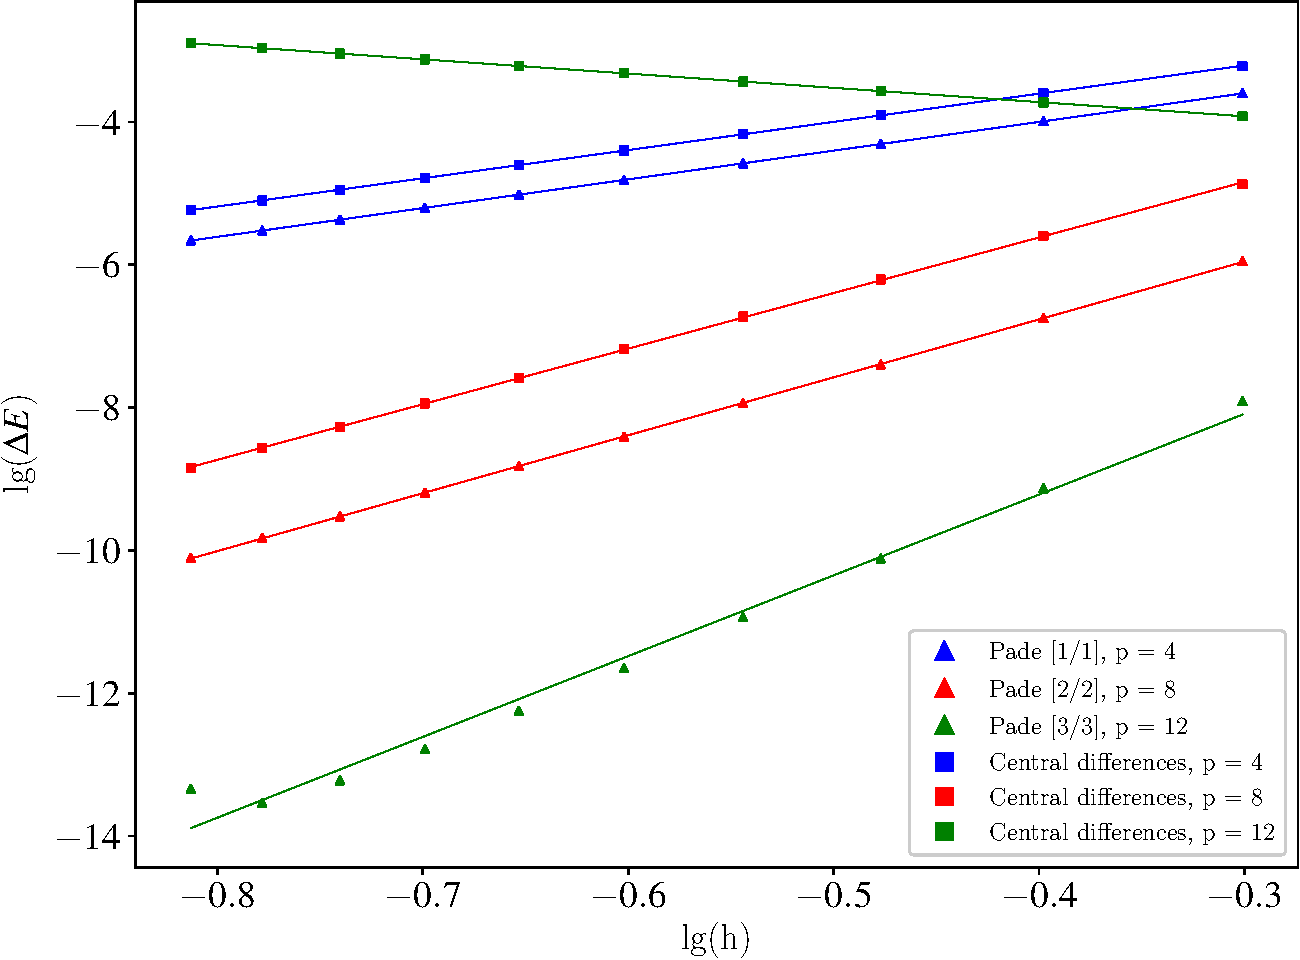
\includegraphics[width=0.8\linewidth]{./pictures/pade_vs_cs-crop.pdf}
        \end{figure}
    \end{block}
\end{frame}

\begin{frame}{Паде аппроксиманты и многоточечные оценки}
    \vspace*{-0.3cm}
    \begin{block}{Гармонический осциллятор, $N = 400$}
        \begin{figure}
            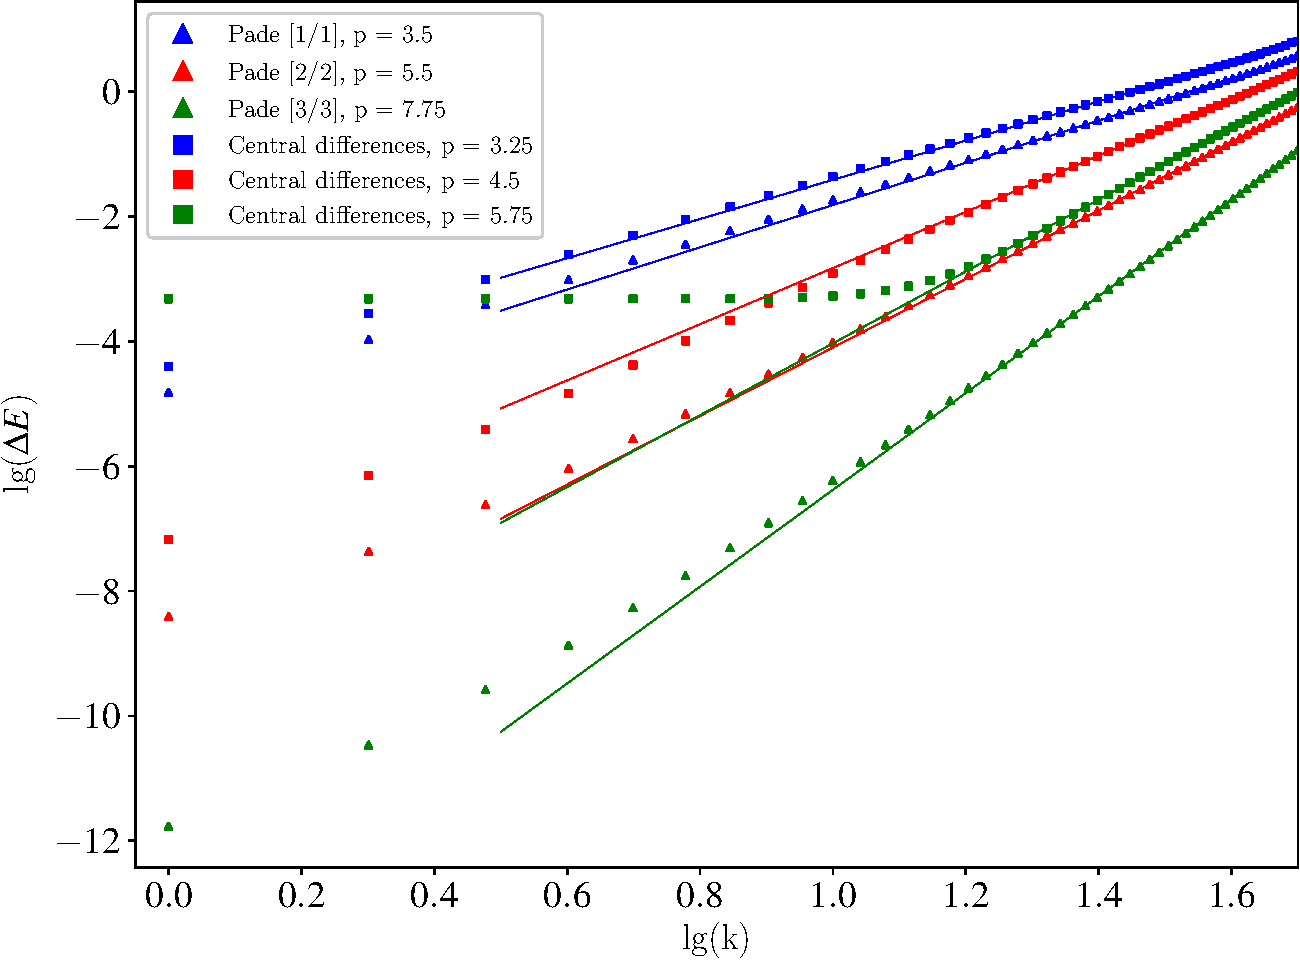
\includegraphics[width=0.8\linewidth]{./pictures/pade_vs_cd_diff_k-crop.pdf}
        \end{figure}
    \end{block}
\end{frame}

\begin{frame}{Колебательно-вращательная задача}
    \vspace*{-0.5cm}
    \begin{gather}
        \lsq -\frac{\hbar^2}{2 \mu} \frac{d^2}{dR^2} + \frac{J(J+1)}{2 \mu R^2} + V(R) \rsq \psi_\text{vib} = E_\text{vib} \psi_\text{vib}, \\
        V(R) = D_e \lb 1 - \exp \lb -a(R - R_e \rb \rb^2 
    \end{gather}
    \vspace*{-0.5cm}
    \begin{figure}[H]
        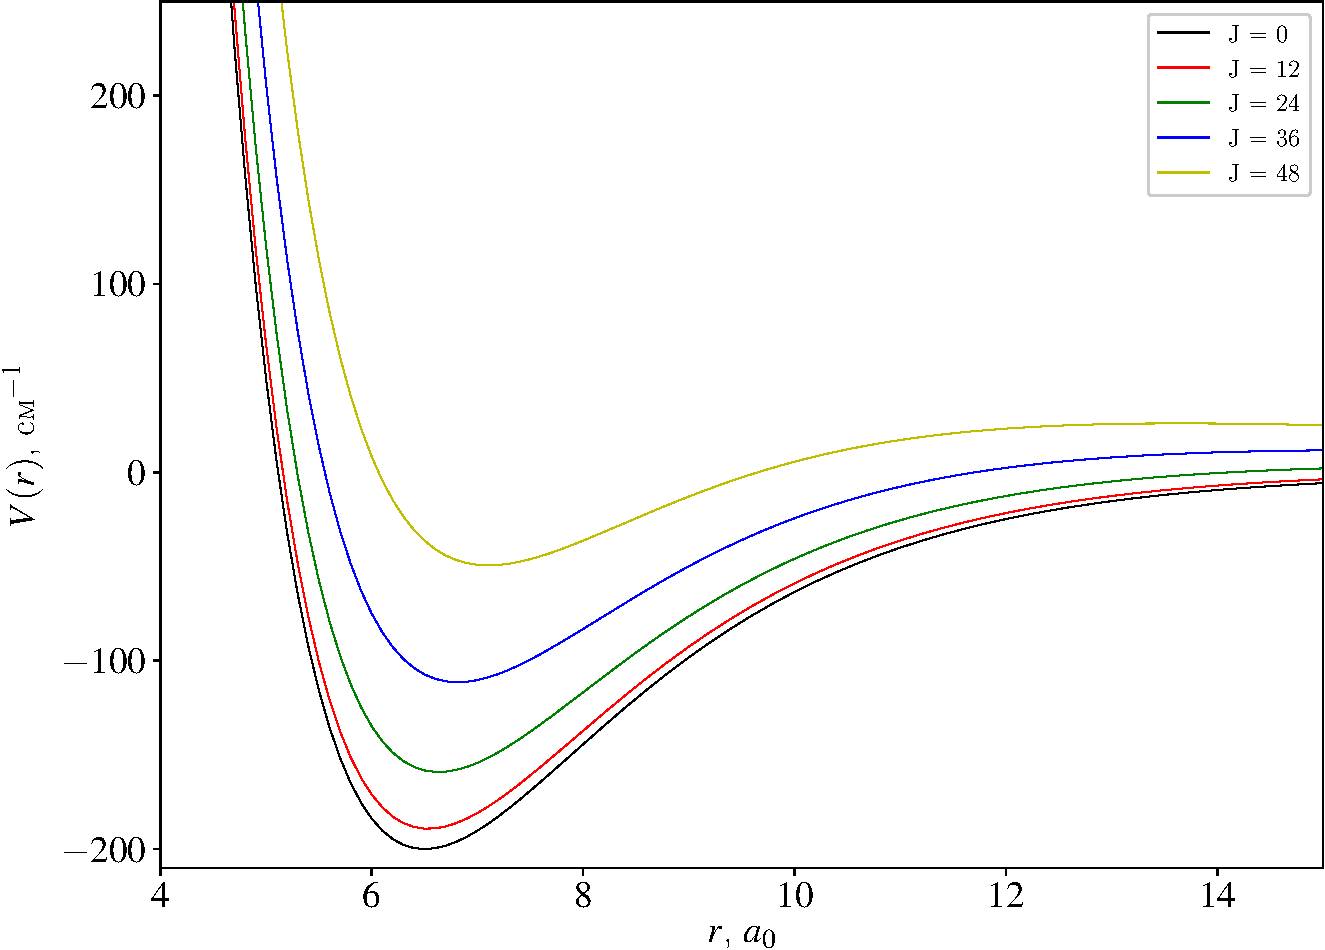
\includegraphics[width=0.7\linewidth]{./pictures/potential_profiles-crop.pdf}
    \end{figure}
\end{frame}

\begin{frame}{Колебательные уровни в потенциале Морзе}
    \begin{block}{}
        \begin{table}[H]
            \vspace*{-0.75cm}
            \caption{Метод Паде [3/3], $J = 0$, $h = 0.25$, $x_0 = 4.0 a_0$, $x_N = 40.0 a_0$}
            \vspace*{-0.25cm}
            \begin{tabular}{ccccc}
             \toprule
             Exact & $\bar{E}_n^{(2)}$ & BOUND & $\Delta E_n$ & $\Delta \bar{E}_n^{(2)}$ \\
             \midrule
                -188.05704228 & -188.05704228 & -188.057042 & $\num{1.847e-12}$ & $\num{1.847e-12}$ \\
                -165.27406801 & -165.27406801 & -165.274068 & $\num{2.245e-12}$ & $\num{2.018e-12}$ \\
                -143.96168198 & -143.96168198 & -143.961682 & $\num{2.672e-12}$ & $\num{3.780e-12}$ \\
                -124.11988418 & -124.11988418 & -124.119884 & $\num{4.533e-12}$ & $\num{9.948e-14}$ \\
                -105.74867462 & -105.74867462 & -105.748674 & $\num{1.228e-11}$ & $\num{7.816e-13}$ \\
                -88.84805329  & -88.84805329  & -88.8480533 & $\num{2.612e-11}$ & $\num{7.816e-13}$ \\
                -73.41802020  & -73.41802020  & -73.4180202 & $\num{4.893e-11}$ & $\num{3.268e-13}$ \\ 
                -59.45857534  & -59.45857534  & -59.4585753 & $\num{8.286e-11}$ & $\num{1.471e-12}$ \\ 
                -46.96971872  & -46.96971872  & -46.9697187 & $\num{1.231e-10}$ & $\num{1.727e-12}$ \\
                -35.95145033  & -35.95145033  & -35.9514503 & $\num{1.632e-10}$ & $\num{6.395e-14}$ \\
                -26.40377018  & -26.40377018  & -26.4037702 & $\num{1.984e-10}$ & $\num{8.775e-13}$ \\
                -18.32667827  & -18.32667827  & -18.3266782 & $\num{2.171e-10}$ & $\num{4.338e-12}$ \\
                -11.72017459  & -11.72017459  & -11.7201746 & $\num{2.152e-10}$ & $\num{7.148e-12}$ \\ 
                -6.58425914   & -6.58425914   & -6.58425915 & $\num{1.901e-10}$ & $\num{8.080e-12}$ \\
                -2.91893193   & -2.91893193   & -2.91893193 & $\num{1.416e-10}$ & $\num{7.269e-12}$ \\
                -0.72419296   & -0.72419296   & -0.72419296 & $\num{6.535e-10}$ & $\num{7.332e-10}$ \\
            \bottomrule                        
            \end{tabular}                      
        \end{table}                            
    \end{block}                                
\end{frame}                                    

\begin{frame}{Колебательно-вращательные уровни в потенциале Морзе}
    \begin{block}{}
        \begin{table}[H]
            \vspace*{-0.75cm}
            \caption{Метод Паде [3/3], $J = 5$, $h = 0.25$, $x_0 = 4.0 a_0$, $x_N = 40.0 a_0$}
            \vspace*{-0.25cm}
            \begin{tabular}{ccc}
                \toprule
                $\bar{E}_n^{(2)}$ & BOUND & $\vert E_n - \bar{E}_n^{(2)} \vert$ \\
                \midrule
 -186.01139971 & -186.0113997   &  $\num{2.842e-14}$ \\  
 -163.31089584 & -163.3108959   &  $\num{1.990e-13}$ \\
 -142.08261657 & -142.0826166   &  $\num{1.080e-12}$ \\
 -122.32674155 & -122.3267416   &  $\num{3.922e-12}$ \\
 -104.04348535 & -104.0434854   &  $\num{1.089e-11}$ \\
 -87.23310751  & -87.23310753   &  $\num{2.458e-11}$ \\
 -71.89592673  & -71.89592674   &  $\num{4.704e-11}$ \\
 -58.03234134  & -58.03234136   &  $\num{7.856e-11}$ \\
 -45.64286031  & -45.64286033   &  $\num{1.168e-10}$ \\
 -34.72815189  & -34.72815190   &  $\num{1.565e-10}$ \\
 -25.28912465  & -25.28912467   &  $\num{1.902e-10}$ \\
 -17.32707277  & -17.32707278   &  $\num{2.100e-10}$ \\
 -10.84396298  & -10.84396300   &  $\num{2.091e-10}$ \\
 -5.84308905   & -5.843089058   &  $\num{1.836e-10}$ \\
 -2.33094799   & -2.330948001   &  $\num{1.339e-10}$ \\
 -0.32590561   & -0.3259056933  &  $\num{6.383e-11}$ \\
            \bottomrule
            \end{tabular}
        \end{table}
    \end{block}
\end{frame}

\begin{frame}{Расчет статистических сумм}
    \begin{block}{Классическая статсумма}
        \begin{gather}
            Q^\text{class}_\text{rovib}(T) = 4 \pi \left( \frac{2 \pi \mu k T}{h^2} \right)^{3/2} \int\limits_\sigma^\infty \frac{\displaystyle \gamma \left( \frac{3}{2}, -\frac{U}{kT} \right)}{\displaystyle \Gamma \left( \frac{3}{2} \right)} \exp \left( -\frac{U}{kT} \right) R^2 d R 
        \end{gather}
    \end{block}
    \begin{block}{Квантовая статсумм}
        \begin{gather}
            Q^\text{q}_\text{rovib}(T) = \sum_{j} (2 J + 1) \exp \lb - \frac{c h E_j}{kT} \rb 
        \end{gather}
    \end{block}
\end{frame}

\begin{frame}{}
    \begin{block}{Отношение статистических сумм}
        \begin{figure}[H]
            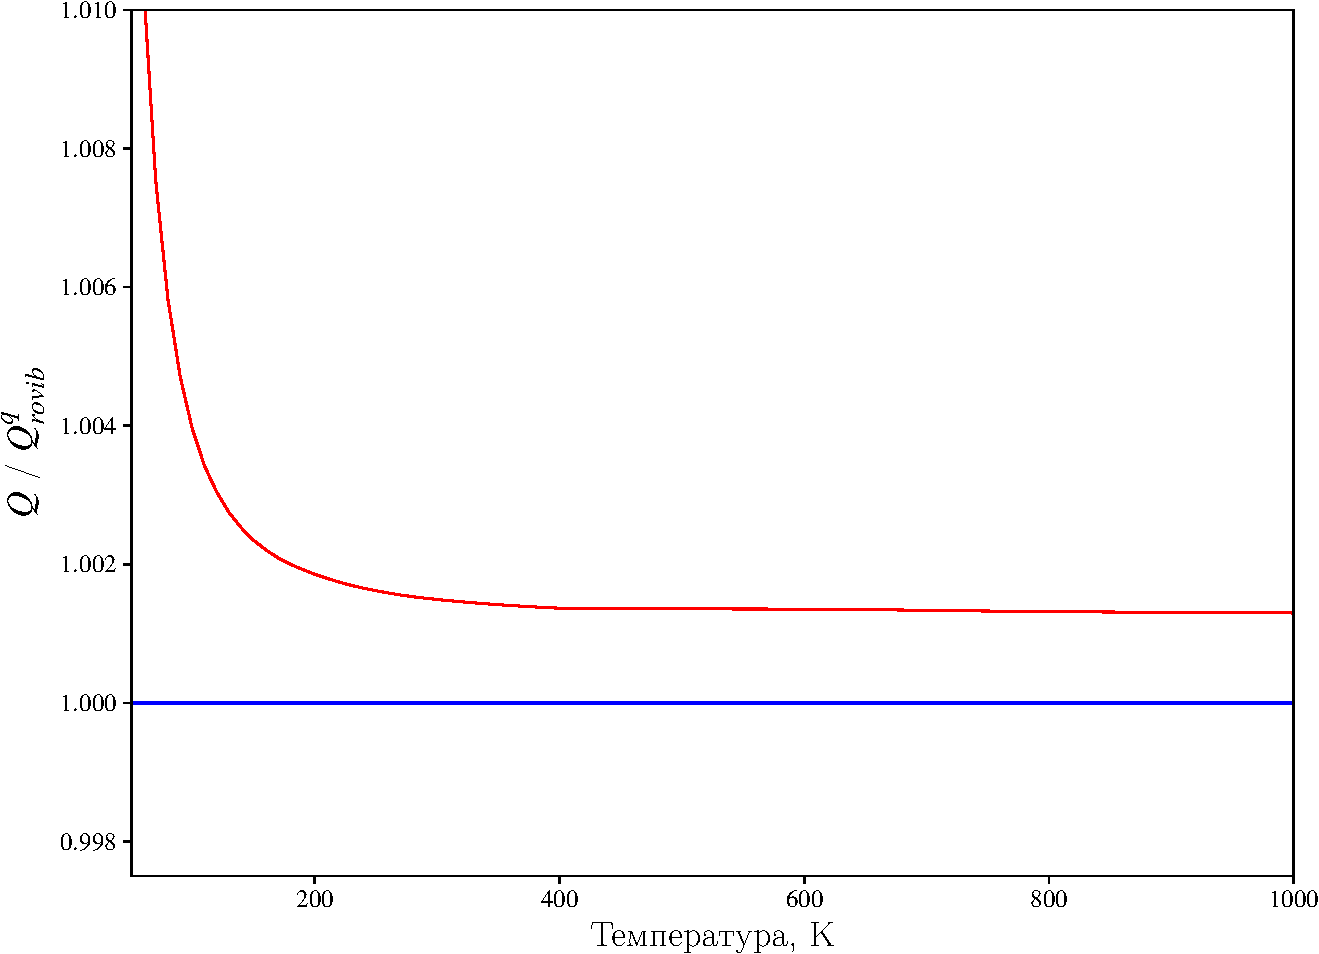
\includegraphics[width=0.8\linewidth]{./pictures/ratio-crop.pdf}
        \end{figure}
    \end{block}
\end{frame}

\end{document}
